\section{Постановка задачи машинного обучения}

Одним из первых, кто дал определение предмету машинного обучения стал американский ученый Артур Самуэль. В 1959 году в своей работе \cite{Samuel:ML}, посвященной созданию искусственного интеллекта по игре в шашки с помощью алгоритма minimax, Артур Самуэль дал определение тому, что есть машинное обучение -- процесс обучения, в результате которого компьютеры способны показывать поведение, которое в них явно не было заложено.

Более современное и точное определение дал Том Митчелл в 1998 году. Корректно поставленная задача обучения определяется следующим образом: говорят, что компьютерная программа обучается на основе опыта E (experience) по отношению к некоторому классу задач T (task) и меры качества P (performance), если качество у задачи из T, измеренное на основе P, улучшается с приобретением опыта E.

Большинство алгоритмов машинного обучения условно можно разбить на несколько классов: обучение с учителем, обучение без учителя, обучение с подкреплением, рекомендательные системы, а также частичное обучение, существуют и другие менее используемые классы алгоритмов.

В алгоритмах обучения с учителем подразумевается обучение на размеченных данных, то есть когда дана матрица, описывающая объекты с помощью признаков (матрица ''объекты-признаки'') и вектор ответов для каждого объекта. Таким образом методы обучения с учителем можно представлять как функциональную зависимость: на каждый набор признаков $x \in X$ есть ответы из $Y$ такие, что $y:~X \rightarrow Y$, где $y$ -- искомая зависимость.

Рассмотрим такой подход более подробно \cite{coursera:voroncov}. Пусть $X$ -- множество объектов, $Y$ -- множество ответов, $y:~X \rightarrow Y$ -- неизвестная зависимость, ставящая в соответствие объекты и ответы.

Пусть также нам известны:\\
\begin{description}[font=$\bullet$]
    \item $\{ x_1, \dots, x_l \} \subset X $ -- известное подмножество объектов;
    \item $y_i,~~\forall~i=\overline{1,n}$ -- известное множество результатов.
\end{description}

Ставится задача найти $a:~X \rightarrow Y$ -- искомый алгоритм, дающий минимальное расхождение с целевой функцией $y$.

Замечание: как правило множество объектов описывается с помощью признаков. Пусть есть $n$ объектов, тогда под признаками объекта будем иметь в виду следующее отображения: $f_j:~X \rightarrow D_j,~~\forall~j=\overline{1,n}$.
Признаки могут быть: количественными $D_j=\mathbb{R}$, бинарными $D_j=\{A, B\}$, номинальными $|D_j|=k<\infty$, упорядочено номинальными. Один объект может задаваться набором признаков разных типов.

Тогда любой объект $x \in X$ может быть описан вектором признаков $(f_1(x), \dots, f_n(x))$.
Следовательно, все объекты можно описать с помощью матрицы ''объекты-признаки'':
$$ F = 
\begin{pmatrix}
f_1(x_1) & f_2(x_1) & \dots & f_n(x_1) \\
f_1(x_2) & f_2(x_2) & \dots & f_n(x_2) \\
\dots    & \dots    & \dots & \dots    \\
f_1(x_l) & f_2(x_l) & \dots & f_n(x_l) \\
\end{pmatrix}
$$
Каждой строчке соответствуют правильные (ожидаемые) ответы, полученные в результате эксперимента, наблюдения, опроса и т.д. По типу представления множества ответов можно разбить на 3 класса:
\begin{description}[font=$\bullet$]
    \item классификация: $Y=\{A,B\},~Y=\{A_1,\dots,A_k\},~Y=\{A,B\}^k$;
    \item регрессия: $Y=\mathbb{R}$ (одномерный случай)$,~Y=\mathbb{R}^k$ ($k$-мерный случай);
    \item ранжирование: в отличие от классификации на множестве $Y$ задано отношение частичного порядка.
\end{description}

Предсказательная модель $a(x)$ строится как параметрическое семейство функций над некоторой фиксированной функцией $g(x)$. Более формально модель $A = \{ a(x) = g(x,\theta) | \theta \in \Theta \}$, где $g:~X \times \Theta \rightarrow Y$ -- фиксированная функция, $\Theta$ -- множество допустимых параметров $\theta$.


В обучении без учителя данные об ответах не известны, поэтому можно говорить лишь о том, как данные расположены друг относительно друга. Данные методы машинного обучения происходят без участия экспериментатора и применяется для обнаружения внутренних взаимосвязей. Обычно так решаются задачи кластеризации, понижения размерности, визуализации данных.

Также используются методы обучения с подкреплением, когда набор данных дается из некоторого потока, а также рекомендательные системы.

Существуют задачи частичного обучения, которые занимают промежуточное положение между задачами регрессии и задачами кластеризации. Задача возникает когда только на части обучающей выборки даны ответы, а другая часть неразмечена, обычно такие задачи возникают при больших объемах данных, когда разметить всю выборку либо невозможно, либо очень дорого. При этом задачи частичного обучения не сводятся ни к классификации, ни к кластеризации.



\section{Методология решения задач машинного обучения}

Вне зависимости от метода машинного обучения задача состоит из 2-х этапов: обучение и применение.
На первой стадии происходит построение оптимального алгоритма $a$ -- функция, дерево, набор инструкций и др. На второй стадии алгоритм выдает ответы для новых объектов.

Оптимальным алгоритмом будем называть такой алгоритм, который на большинстве объектов обучающей выборки дает правильные ответы или достаточно близкие ответы к ожидаемым. Для того чтобы это сделать нужно определять точность или расстояние между объектами, другими словами нужно задать метрику в пространстве объектов. Для этого вводится понятие функции потерь $\mathfrak{L}$ -- величина ошибки алгоритма $a \in A$ на объекте $x \in X$:
\begin{description}[font=$\bullet$]
    \item $\mathfrak{L} (a,x)=
    \begin{cases}
        1, &\text{если $a(x) \neq y(x)$,}\\
        0, &\text{иначе.}
    \end{cases}
    $ -- индикатор ошибки для случая классификации;
    \item $\mathfrak{L} (a,x)= |a(x) - y(x)|^p$ -- для случая регрессии.
\end{description}

%Замечание: при $p=1$ для регрессии функция ошибки берется как модуль разности алгоритма и ответа.

На практике для случая регрессии обычно берут $p=2$ т.к. при $p=1$ возникает проблема с дифференцированием функции потерь. Однако, если в выборке присутствуют большие по модулю выбросы, то можно брать $p=1$, поскольку тогда модель будет меньше реагировать на большие отклонения.

Чтобы в целом оценить алгоритм берут сумму функций потерь по всем объектам из обучающей выборки, деленную на ее мощность, получившуюся величину называют эмпирическим риском (функционал качества алгоритма $a$ на объектах $X^l$): $Q(a, X^l) = \dfrac{1}{l}\sum\limits_{i=1}^{l}\mathfrak{L}(a,x_i)$.

Таким образом, задача обучения сводится к задаче оптимизации (минимизация функционала эмпирического риска на обучающей выборке): $\mu(X^l) = \arg\min\limits_{a \in A} Q(a,X^l)$.

Замечание: иногда сумму делят не на $l$, а на $2 \cdot l$, с той целью, чтобы при дифференцировании функции эмпирического риска сократились некоторые коэффициенты (для $p=2$).

Для решения задачи минимизации применяют различные численные методы. Например, метод наименьших квадратов (МНК).


\subsection{CRISP-DM}

\begin{wrapfigure}{r}{0.45\linewidth} 
    \vspace{-2ex}
    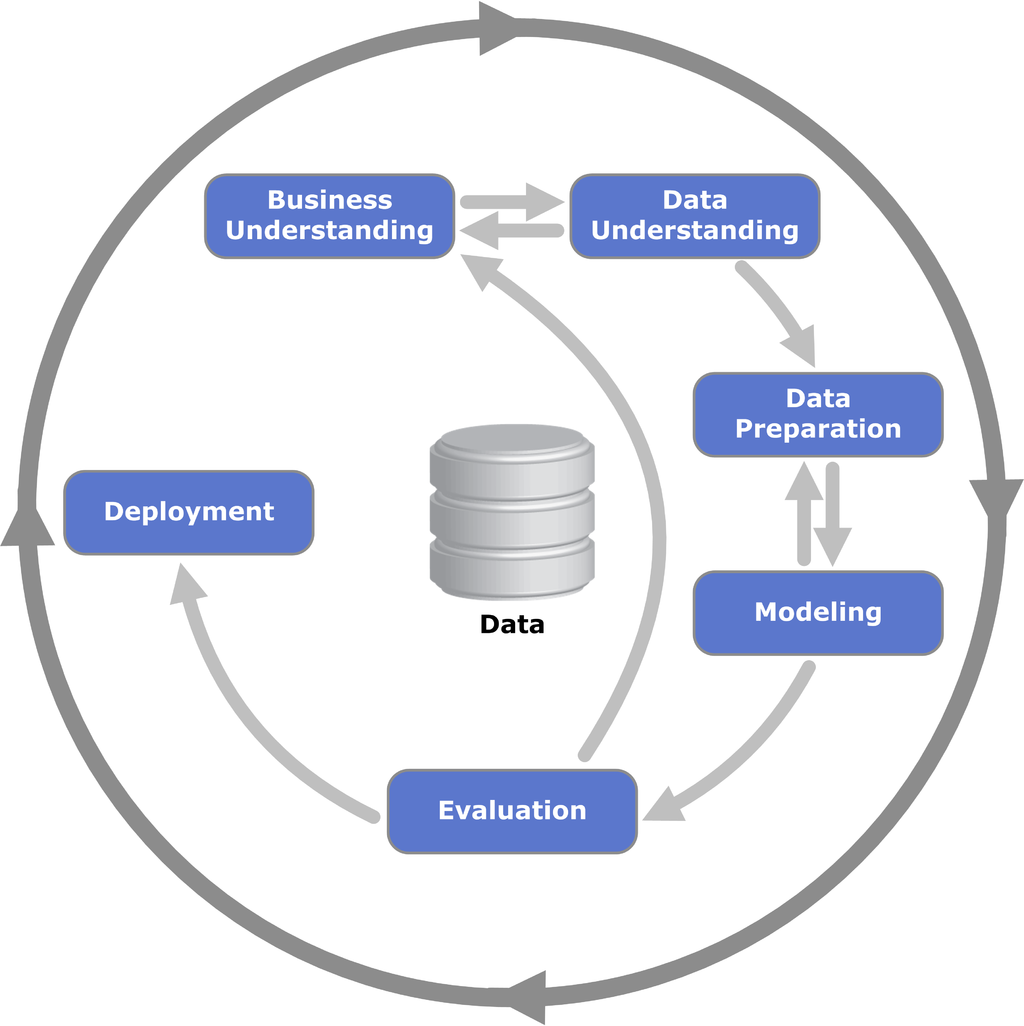
\includegraphics[width=\linewidth]{src/img/CRISP-DM_process_diagram.png}
    \caption{Жизненный цикл исследования данных \cite{wiki:crisp_dm}}
    \label{fig:crisp_dm}
\end{wrapfigure}

Таким образом, любая задача машинного обучения: классификация, регрессия, кластеризация сводится к оптимизационной задаче, возможно с ограничениями. По этой причине были предприняты попытки по созданию единого алгоритма решения задач. Чтобы облегчить процесс решения задач, был разработан и предложен CRISP-DM (CRoss Industry Standard Process for Data Mining) -- межотраслевой стандарт решения задач интеллектуального анализа данных. CRISP-DM -- модель жизненного цикла исследования данных.
Первая версия данного стандарта была принята в 1999 году. Стандарт призван формализовать схему решения задач анализа данных. Предлагается алгоритм решения произвольной задачи анализа данных в 5 шагов, причем они могут замыкаться в цикле.

\begin{enumerate}[label=\arabic*.]
    \item Вначале исследователь должен понять предметную область или сферу бизнеса;
    \item Далее необходимо понять как собирались данные;
    \item На следующем шаге нужно определить есть ли в данных шумы, пропуски, выбросы, все ли признаки несут полезную информацию, можно ли вычислить полезные признаки по уже имеющимся, данный этап можно назвать подготовкой данных;
    \item После происходит моделирование или построение предсказательной модели;
    \item Полученная модель оценивается с помощью выбранных метрик;
    \item Если качество полученной модели удовлетворяет исследователя, модель внедряется в производственные процессы и эксплуатируется.
\end{enumerate}
Помимо CRISP-DM существуют менее известные стандарты: My own, SEMMA и другие. На сайте \cite{poll:crisp_dm} публикуются результаты опросов по популярности методологий анализа данных.



\section{Методы оптимизации}

Во многих задачах науки, экономики и бизнеса возникают проблемы нахождения экстремальных значений целевой функции. При этом на множество допустимых решений могут быть наложены ограничения. Такие задачи называются задачами оптимизации. Если есть ограничения, то говорят о задаче условной оптимизации, иначе безусловной оптимизации. Рассмотрим некоторые методы решения задач оптимизации.


\subsection{Градиентный спуск}

Метод градиентного спуска является наиболее часто используемым методом ввиду быстроты работы для большинства задач и многообразия модификаций метода (метод наискорейшего спуска, метод сопряженных градиентов, метод Нестерова, метод стохастического спуска и многие другие)
Для отыскания экстремальной точки в градиентном спуске используют итеративную формулу:
$$ x := x - \alpha \nabla f(x) $$

Где $\nabla f(x)$ -- градиент функции $f(x)$, в векторной форме градиент можно записать как $\nabla f(x) = \frac{\partial f(x)}{\partial x_1} \vec{i_1} + \frac{\partial f(x)}{\partial x_2} \vec{i_2} + \dots + \frac{\partial f(x)}{\partial x_n} \vec{i_n}$, причем $\vec{i_1}, \vec{i_2}, \dots, \vec{i_n}$ - единичные векторы. Направление градиента указывает на то направление из точки $x$, которое имеет наибольшую скорость роста функции из данной точки. Соответственно, антиградиент $-\nabla f(x)$ показывает направление наискорейшего убывания;

$\alpha$ -- шаг градиента (в машинном обучении называют скоростью обучения). Данный параметр выбирается вручную, при этом, если $\alpha$ мал, то методу потребуется много итераций для сходимости, если же $\alpha$ большой, то метод градиентного спуска может начать расходится, то есть значение $x$ будет отдалятся от точки экстремума. Существует условие Липшица \cite{habr:grad_descent}, которое дает достаточное условие сходимости градиентного спуска: если $\exists L:~\forall x, y \hookrightarrow || \nabla f(x) - \nabla f(y) || \leq L || x - y ||$, то для $\forall \alpha < \frac{2}{L}$ гарантируется убывание функции $f(x)$. На практике обычно выбирают $\alpha=10^{-2}$, либо еще меньше в зависимости от того, какая точность необходима.

\begin{wrapfigure}{r}{0.45\linewidth} 
    \vspace{-3ex}
    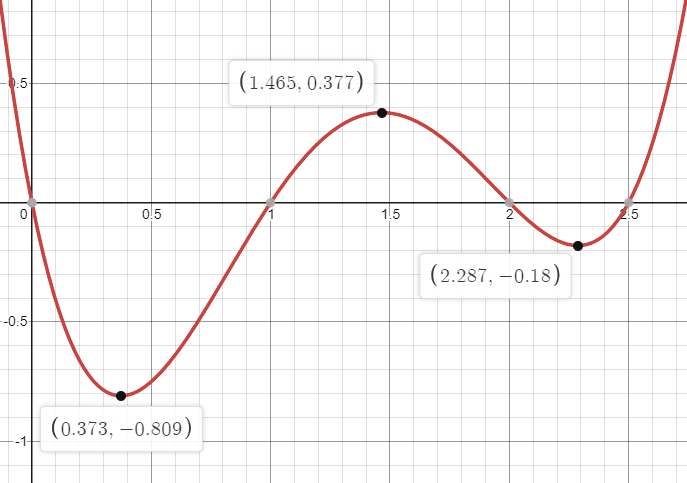
\includegraphics[width=\linewidth]{src/img/multi_extreme.png}
    \caption{Проблема много экстремальности функции}
    \label{fig:multi_extreme}
\end{wrapfigure}

Важной особенностью градиентных методов является выбор начального приближения $x_0$, так, если производится поиск минимума и функция имеет несколько минимумов, как на рисунке \ref{fig:multi_extreme}, то выбор $x_0$ будет определять найденный минимум. Например, если $x_0 = 2$, метод найдет минимум $f(x^*) = -0.18$, если $x_0 = 1$, то $f(x^*) = -0.809$, если же $x_0 = 1.5$, то метод не сможет найти ни один минимум функции, поскольку в точке $x = 1.5$ производная функции $f(x)$ равна 0, поэтому $\nabla f(x) = 0$ и формула градиентного спуска вырождается в $x := x$. Для того чтобы метод искал глобальный минимум можно запустить данный метод несколько раз из разных начальных точек. Выбрать начальные приближения можно как самому, так и выбрать их случайным образом из равномерного распределения на отрезке $[ a, b ]$. Для проверки того, что был найден глобальный минимум можно запустить метод из точек $x^* - x_L,~x^* + x_L$, где $x^*$ -- найденный минимум, $x_L$ -- точка с большими по модулю координатами. Если метод не сойдется к тому же решению, то необходимо сравнить 2 минимума и выбрать наименьший.

При поиске экстремума в овражных функциях градиентный спуск сходится медленно, причем если число аргументов функции велико, то довольно часто можно встретить овражные области. Для решения данной проблемы используют модификации градиентного спуска, так называемые, овражные методы.

Для ускорения сходимости градиентного спуска применяют различные техники. Можно определять $\alpha$ на каждом шаге по следующей формуле: $\alpha_{k} = \arg \min\limits_{\alpha \in \left[  0, \infty \right) } f(x^k - \alpha f'(x_k))$ метод с таким выбором градиентного шага носит называние метода наискорейшего спуска, также можно уменьшать параметр $\alpha$ на каждом шаге. Идея заключается в том, что после каждого шага расстояние до экстремума уменьшается, следовательно, нужно уменьшить градиентный шаг.


\subsection{Инерционный градиентный спуск}

Метод известен с середины 20 века и изначально носил название метод тяжелого шарика. Идея данного метода -- добавить в формулу градиентного спуска свойство инерционности, то есть чтобы на каждом следующем шаге аргумент $x_{k+1}$ зависел не только от значения антиградиента, но и также от значения предыдущего шага. Для этого предлагается добавить в формулу градиентного спуска следующее слагаемое $\beta (x_k - x_{k-1})$, где $\beta$ -- коэффициент инерции, также как и $\alpha$ является гиперпараметром, то есть задается вручную. Как правило коэффициент инерции берется немного меньше единицы.

Все семейство инерционных градиентных методов можно описать следующей формулой:
$$ x_{k+1} = x_k - \alpha_k \nabla f(x_k) + \beta_k (x_k - x_{k-1}) $$

Добавление нового слагаемого в метод градиентного спуска не меняет асимптотической сложности алгоритма, при этом, если выбрать оптимальные значения в паре $(\alpha_k, \beta_k)$, можно добится ускорения метода на порядок.


\subsection{Стохастический градиентный спуск}

Идея метода заключается в использовании вместо градиента функции $\nabla f(x)$ другую функцию (случайный процесс) $g(x,\theta)$ такую, что математическое ожидание $E[g(x,\theta)] = \nabla f(x)$, где $\theta$ -- случайная величина.
Метод стохастического градиента можно описать следующей формулой:
$$ x_{k+1} = x_k - \alpha_k g(x_k,\theta_k) $$

Если $x$ -- вектор с большим количеством компонент, то вычисление градиента может происходить продолжительное время. Поэтому если использовать метод стохастического градиента и в качестве $\theta$ взять случайный индекс у $x$, то есть $x_i$, где $i$ -- случайная величина, то вычисление градиента сведется к вычислению частной производной по аргументу со случайным индексом. За счет этого происходит существенное ускорение сходимости, это называется процедурой Роббинса-Монро и Кифера–Вулфовица, представленные в 1951 и 1952 годах соответственно \cite{wiki:stochastic_grad}. В настоящее время данный метод активно применяется в алгоритмах машинного обучения и в нейронных сетях, где количество признаков у объектов может быть велико. Следует сказать, что данный метод реализован в крупных библиотеках машинного обучения: TensorFlow, PyTorch. Метод используется для обучения моделей с большим и сверх большим объемом данных из-за того, что даже на небольшой подвыборке объектов модель может хорошо обучиться.


\subsection{Нормальное уравнение (Normal Equation)}

Нормальное уравнение позволяет найти экстремум функционала аналитически, без необходимости применять итеративный подход. Пусть функционал задан следующим образом: $\mathfrak{L}(\theta_1,\theta_2,\dots,\theta_m) = \frac{1}{2m} \sum\limits_{i=1}^{m}(h_{\theta}(x^{(i)}) - y^{(i)})^2$ поставим задачу минимизации этого функционала по всем параметрам $\theta$, при условии, что известны $m$ пар $(x^{(i)}, y^{(i)})$. Составим из $x^{(i)}$ матрицу: $X = (x^{(1)}, x^{(2)}, \cdots, x^{(m)})$, тогда $\theta = (X^{T} X)^{-1} X^{T} y$.

В отличии от градиентных методов в данном методе не нужно проводить итерационную процедуру, а также в методе отсутствуют гиперпараметры. Однако для вычисления ответа нужно вычислить обратную матрицу порядка $n \times n$, алгоритм вычисления обратной матрицы работает за $O(n^3)$ по времени, поэтому для объектов с большим числом признаков, например $n=10^6$ потребуется $C \cdot 10^{18}$ операций, где $C$ -- некоторая константа из алгоритма обратной матрицы. Современные компьютеры могут обрабатывать порядка $10^9$ операций в секунду, учитывая нужное количество операций алгоритм не успеет за разумное время вычислить минимум функции. Поэтому область применимости метода -- объекты с небольшим числом параметров $(< 10^4)$. На объектах с большим числом признаков хорошо работает стохастический градиентный спуск.



\section{Регрессионный анализ}

Задача регрессионного анализа состоит в определении наиболее оптимальной функции $f(x)$, которая бы наилучшим образом восстанавливала закономерность во входных парах данных $(x_i, y_i)$. Тогда можно записать следующее соотношение: $y = f(x) + \varepsilon$, где $f(x)$ -- функция, предсказывающая поведение $y$, $\varepsilon$ -- случайная величина с нулевым математическим ожиданием. В большинстве задач полагается, что $\varepsilon$ имеет нормальное распределение.

Задача исследователя состоит в определении вида функции $f(x)$. После происходит параметризация данной функции, выбирается функция штрафа за отклонение от целевого значения, например, сумма квадратов отклонений. Нахождение оптимальных параметров $\theta$ означает минимизацию функции потерь. Таким образом задача регрессии сводится к задаче оптимизации. Рассмотрим конкретные виды аппроксимирующих моделей.


\subsection{Линейные модели}

Иногда, искомую зависимость можно хорошо аппроксимировать линейными моделями, например это могут быть: прогноз стоимости дома или квартиры, классификация типа опухоли, предсказание оттока клиентов, прогноз оклада по описанию вакансии, некоторые физические законы (Гука, Ома, Паскаля).


\subsubsection{Линейная регрессия}

Модель линейном регрессии называется так из-за того, что функция прогноза выглядит как линейная комбинация компонент объекта и компонент вектора параметров. Пусть $f(x,\theta) = \sum\limits_{i=1}^N x_i \theta_i = (\theta, x)$. Чтобы записать последнее равенство в вектор $x$ добавляют фиктивную компоненту, равную единице для того, чтобы размерности вектора параметров и вектора объекта совпадали. В качестве функции штрафа можно взять, например $SSE = \sum\limits_{i=1}^N  (y_i - f(x_i,\theta))^2 = \sum\limits_{i=1}^N  (y_i - (\theta, x_i))^2$. Тогда, определив, с помощью методов теории оптимизации, вектор $\theta$, будет найдена искомая функция.

В общем случае можно считать что модель $f(x,\theta)$ задает гиперплоскость в $n$-мерном пространстве и чем больше расстояние объекта до гиперплоскости тем больше штраф.

Если среди признаков есть линейно зависимые, то модель теряет свою точность на тестовой выборке, хотя на обучающей выборке можно достичь максимальной точности. Данная проблема называется мультиколлинеарностью линейной модели. При этом возможны 2 случая: функциональная зависимость, когда набор признаков однозначно и точно определяет другой признак и частичную мультиколлинеарность, когда линейная комбинация части признаков сильно коррелирует с другим признаком. При функциональной зависимости вектор параметров определяется неоднозначно, следовательно появляется степень свободы при выборе параметров и можно подобрать их так, чтобы на тестовой выборке они давали завышенные метрики качества. Частичная мультиколлинеарность приводит к неустойчивости оценок.

Существует несколько способов борьбы с мультиколлинеарностью: 
\begin{description}[font=$\bullet$]
    \item Метод главных компонент -- позволяет уменьшить размерность пространства признаков и следовательно избавиться от их коррелированности;
    \item гребневая регрессия -- добавим в функционал эмпирического риска штрафное слагаемое за большие по модулю значения вектора параметров: $Q = \frac{1}{N} \mathfrak{L}(\theta,x_i,y_i,f) + \frac{\tau}{2}|| \theta ||^2$, где $\tau$ -- коэффициент регуляризации. При минимизации $Q$ будет минимизироваться как сумма функций потерь, так и квадрат нормы вектора параметров. Подбор параметра $\tau$ можно сделать вручную, посмотрев на качество метрик на текстовой выборке или определить по критерию скользящего контроля;
    \item метод LASSO -- (Least Absolute Shrinkage and Selection Operator) в отличие от гребневой регрессии, в методе LASSO берется сумма модулей компонент вектора параметров: $Q = \frac{1}{N} \mathfrak{L}(\theta,x_i,y_i,f) + \tau\sum\limits_{i=1}^N |\theta_i|$, также некоторые значения $\theta_j$ могут стать в точности нулем, следовательно соответствующий признак больше не будет учитываться. Таким образом в данном методе происходит отбор признаков.
\end{description}

Гребневая регрессия и метод LASSO позволяют ограничить вектор параметров и тем самым избежать проблемы мультиколлинеарности, при этом в методе LASSO можно провести селекцию признаков то есть убрать часть из них.

Говорят, что регуляризация приводит к сокращению размерности пространства, хотя само пространство остается той же размерности, сокращается эффективная размерность, поскольку мы накладываем на вектор параметров ограничение.


\subsubsection{Полиномиальная регрессия}

Линейная регрессия требует чтобы между целевой переменной и переменными признаков была линейная зависимость. На практике возникают случаи, когда зависимость между данными невозможно описать линейным образом, для этого рассмотрим модель регрессии с полиномом. Определим модель следующего вида: $f(x,\theta) = \sum\limits_{i=0}^k \theta_i x^i = \theta_0 + \theta_1 x + \theta_2 x^2 + \dots + \theta_k x^k $. Тогда $f$ задает полиномиальную регрессию. При этом $x$ может быть как скалярной величиной, так и векторной. Такая модель все еще остается линейной так как степени при весах остаются первого порядка. Следует отметить, что полиномиальная регрессия может привести к эффекту переобучения, если наибольшая степень $k$ будет высокой, поскольку выразительная способность (число степеней свободы) модели будет велико, то модель сможет подстроиться под имеющие данные и не будет обладать обобщающей способностью.


\subsubsection{Пуассоновская регрессия}

Пуассоновская регрессия применяется, когда целевая переменная имеет пуассоновское распределение или в основе которой лежат события, счетчиком которых она является. При этом частота возникновения событий не обязательно стационарна, а может меняться со временем. Пуассоновское распределение имеют, например количество звонков в колл-центр за период времени или число вакцинированных людей за период времени. Для описания частотности событий введем обозначение: $\lambda$, которое возможно зависит от времени.

Пуассоновская регрессия основывается на Пуассоновском распределении, которое имеет следующее распределение вероятности: $p(k) = \dfrac{e^{-\lambda t} (\lambda t)^k}{k!}$ -- вероятность получения $k$ событий за время $t$ с интенсивностью потока $\lambda$. Математическое ожидание распределения Пуассона численно равно интенсивности потока $\lambda$, следовательно для интервала времени $[0, t]$ можно ожидать $\lambda t$ событий.

Если целевая переменная определяется распределением Пуассона и нет оснований говорить о нестационарности потока событий, в качестве оценки можно использовать значение интенсивности потока $\lambda$.

Если же $\lambda$ может изменяться от одного события к другому, то предполагается, что $\lambda$ зависит от объясняющих признаков по некоторому закону. Задача регрессии в таком случае состоит в приближении значений целевой переменной $y$ к $\lambda(x)$. Для этого функция гипотезы $\lambda(x)$ параметризуется. Как правило \cite{Ignatov:functional_dependence} $\lambda(x, \theta) = e^{x \cdot \theta}$, где $\theta$ -- вектор обучаемых параметров, $x$ -- вектор признаков, описывающих объект.

Таким образом вероятность обнаружить $y_i$ событий для объекта $x_i$ равна условной вероятности $p(y_i | x_i ; \theta) = \dfrac{e^{-\lambda_i(x, \theta)} \lambda_i^{y_i}(x, \theta)}{y_i!}$.

Для нахождения $\theta$ воспользуемся методом максимального правдоподобия (ММП). Функция правдоподобия имеет следующий вид: $L(\theta | X, y) = \prod\limits_{i=1}^{N} p(y_i | x_i; \theta) = \prod\limits_{i=1}^{N} \dfrac{e^{-\lambda_i(x, \theta)} \lambda_i^{y_i}(x, \theta)}{y_i!}$.

Максимизируем полученное выражение по $\theta$ (переменная $\lambda_i$ зависит от $\theta$), для удобства будем максимизировать не $L(\theta | X,y)$, а $l(\theta | X,y) = \ln L(\theta | X,y)$ на значение максимума это не повлияет, поскольку логарифмическая функция монотонно возрастающая. Данное преобразование удобно тем, что при вычислении производной удобнее считать производную суммы, чем производную произведения. По свойству логарифма произведения: $l = \sum\limits_{i=1}^{N} \ln \left( \dfrac{e^{-\lambda_i(x, \theta)} \lambda_i^{y_i}(x, \theta)}{y_i!} \right) = \sum\limits_{i=1}^{N} \left( -\lambda_i(x, \theta) + y_i \ln(\lambda_i(x, \theta)) - \ln(y_i!) \right)$. Функция $l$ называется логарифмической функцией правдоподобия. Найдя максимум этой функции по $\theta$ одним из численных методов, получим такие значения $\theta$, которые при подстановке в исходную функцию правдоподобия максимизируют ее.

В данном методе метрикой качества является значение функции максимального правдоподобия. Та модель лучше, у которой большее значение функции, учитывая, что эффекта переобучения нет, либо его влиянием можно пренебречь.

Когда модель обучилась, то есть подобран вектор параметров для получения прогноза количества событий для объекта $x_{predict}$ вычисляется значение $\lambda(x_{predict}, \theta)$, далее искомая величина $y_{predict}$ вычисляется по следующей формуле: $y_{predict} = \arg\max\limits_{k \in \mathbb{Z}^+} p(k | x_{predict}, \theta)$.

Помимо Пуассоновской регрессии существуют и другие модели, основанные на подсчетах: модель Пуассона с нулевым завышением, отрицательная биномиальная регрессия, обобщенная Пуассоновская регрессия \cite{towardsdatascience:poisson_regression}.


\subsubsection{Геометрическая регрессия}

Геометрическая регрессия применяется, когда целевая функция имеет геометрическое распределение. Функция вероятности первого 'успешного' испытания в серии Бернулли с $n$ повторениями и вероятностью 'успеха' $p$ имеет вид: $P(X=n)=(1-p)^{n}p$, где $p$ -- некоторая функция, выбираемая исследователем, причем на данных из набора данная функция должна принимать значения от нуля до единицы, из-за вероятностных ограничений. Для нахождения $\theta$ воспользуемся ММП. Функция правдоподобия имеет следующий вид: $L(\theta | X,y) = \prod\limits_{i = 1}^N (1-p(x_i,\theta))^{y_i}p(x_i,\theta)$.

Используя численные методы вычислим максимум полученной функции, однако для удобства будем искать максимум не $L(\theta, X, y)$, а $l(\theta | X,y) = \ln L(\theta | X,y)$. Тогда функция логарифмического правдоподобия будет иметь следующий вид: $l(\theta, X, y) = \sum\limits_{i = 1}^N ( y_i \ln(1 - p(x_i,\theta)) + \ln(p(x_i,\theta)) )$.

Как и в модели пуассоновской регрессии метрикой качества является значение функции максимального правдоподобия. Та модель лучше, у которой большее значение функции, учитывая, что эффекта переобучения нет, либо его влиянием можно пренебречь.

Когда модель обучилась, то есть подобран вектор параметров для получения прогноза количества событий для объекта $x_{predict}$ вычисляется значение $p(x_{predict}, \theta)$, далее искомую величину $y_{predict}$ можно вычислить по следующей формуле: $y_{predict} = \dfrac{1}{p(x_{predict}, \theta)}$.

\subsubsection{Проблема переобучения и метрики качества}

Проблема переобучения или эффект переподгонки -- одна из самых частых проблем машинного обучения. Данная проблема возникает, когда модель очень сильно подстроилась под объекты на обучающей выборке и из-за этого потеряла обобщающую способность. Эффект можно обнаружить, если сопоставить функции эмпирического риска, вычисленные для обучающей и тестовой выборок, тогда на значение функционала на обучающей выборке будет близко к нулю, а значение на тестовой выборке будет существенно больше.

\begin{wrapfigure}{r}{0.45\linewidth} 
    \vspace{-2ex}
    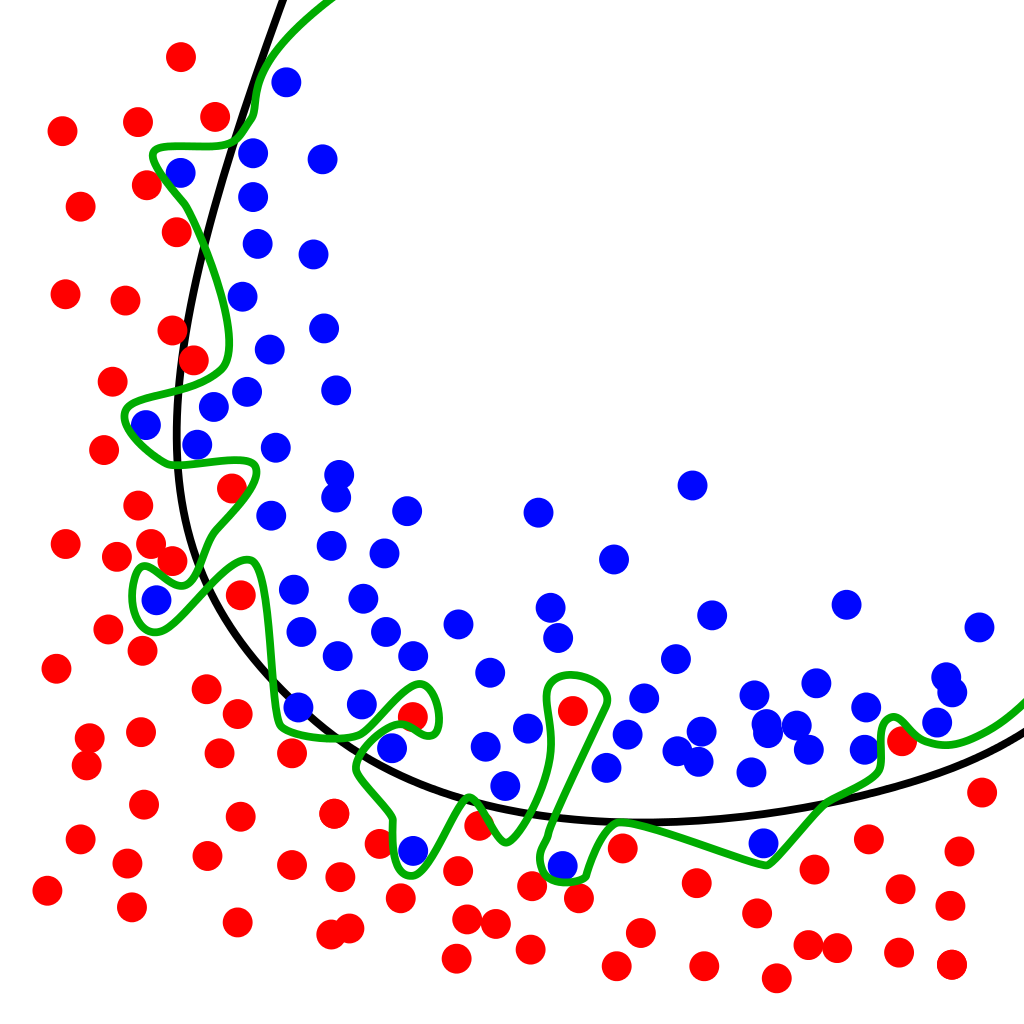
\includegraphics[width=\linewidth]{src/img/wiki_overfitting.png}
    \caption{Пример переобучения модели \cite{wiki:overfitting}}
    \label{fig:wiki_overfitting}
\end{wrapfigure}

На рисунке \ref{fig:wiki_overfitting} изображены две кривые, соответствующие двум модели, решающие задачу классификации. Видно, что черная разделительная кривая классифицирует данные более общо, чем зеленая кривая. Можно говорить, что модель с зеленой разделительной кривой переобучена. Эффект связан с тем, что в выборке существуют случайные отклонения, которые могут быть обусловленны ошибкой измерения или погрешностью, при этом, если модель обладает высокой выразительной способностью, она настраивается на этих данных, что приводит к ухудшению качества на тестовой выборке.

Для того чтобы измерять эффект переобучения считают функционалы, измеряющие качество построенной модели на данных на которых модель не обучалась. 

Рассмотрим 3 таких метода:
\begin{description}[font=$\bullet$]
    \item Отложенная выборка (hold-out) -- деление всей выборки на 2 части (обучающая и валидационная). Недостатком данного функционала качества является то, что можно неудачно сделать разбиение так, что оценка будет смещенной, субъективной. Важным параметром данного метода является отношение размеров разбиений, если обучающая выборка мала, оценка качества будет пессимистической, если же валидационная выборка мала, оценка будет неточной. В большинстве случаев обучающую выборку берут в размере 70-80\% от общего размера;
    \item Скользящий контроль (leave-one-out) -- по очереди будем выбирать один объект из выборки, на оставшейся части будем обучаться, а на выбранном объекте тестировать. После результаты тестирований усредняются. Таким образом невозможно получить смещенную выборку как в hold-out, однако обучение нужно проводить столько же раз, сколько объектов в обучающей выборке;
    \item Кросс-валидация (cross-validation) -- выберем число групп $N$, примерно одинакового размера, равномерно распределим объекты выборки по группам. После будем проводить обучение на $N-1$ группе, а тестирование на оставшейся. Результаты усредняются. При выборе малого числа групп оценки будут пессимистичными, но при этом точными. При большом числе групп оценки будут несмещенными, но с большой дисперсией. Обычно выбирают число групп от 5 до 10.
\end{description}
Данные методы основываются на предположении об одинаковости распределении в группах данных и их независимости. Если данные зависимы или их можно разбить на группы так, чтобы в разных группах распределение были разными, возникает риск переобучения.

Также потеря качества может возникнуть при неправильном проведении отбора признаков или понижения размерности. Корректно в начале разбить выборку на обучающую и валидационную, а отбор признаков или понижение размерностей необходимо проводить не над всей выборкой, а только над обучающей. После проводится проверка качества на валидационной выборке. Было бы ошибочно проводить отбор признаков или понижение размерности на всей выборке до разбиения.


\subsection{Нелинейные модели}

Нелинейные модели регрессии -- такие методы регрессионного анализа, в котором в моделирующей функции параметры модели входят нелинейным образом.


\subsubsection{Решающие деревья}

Данный метод исходно разрабатывался для решения задач классификации, однако в настоящее время существует алгоритм CART, расширяющий класс решаемых задач методом решающих деревьев на случай регрессии, поэтому данный метод помещен в раздел "Регрессионный анализ".

Решающие деревья -- попытка формализовать человеческое мышление при принятии решений. Решающее дерево можно приближенно проиллюстрировать на примере работы врача: врач задает пациенту уточняющие вопросы, исходя из его ответов происходит спуск по дереву на уровень ниже. Вершина, в которую нужно перейти определяется ответом на вопрос. Если у вершины нет дочерних вершин, она листовая в данном примере листовые вершины -- диагноз больного или совет. Таким образом за конечное количество вопросов можно дойти от корневой вершины до листовой.

Все вершины дерева можно разделить на листовые и внутренние. Любая внутренняя вершина $v$ содержит предикат $\beta_v : X \rightarrow A$, для случая бинарного решающего дерева $A = \{0, 1\}$. Любая листовая вершина $v$ содержит метку класса $c_v$.

Для построения решающего дерева используется алгоритм Induction of Decision Tree (ID3). На вход алгоритм может принимать часть выборки U.

\begin{code}
\begin{minted}[fontsize=\footnotesize]{python}
def LearnID3(U):
  if все объекты из U лежат в одном классе:
    return (новый лист v, c_v = c)
  найти предикат с максимальной информативностью beta = argmax I(beta,U)
  разбиваем выборку на U0 и U1 по предикату beta
  if len(U0) == 0 or len(U1) == 0: # не смогли найти информативный предикат
    return (новый лист v, c_v = мажоритарный_класс(U))
  создать новую вершину v
  построить левое  дерево: L_v = LearnID3(U0)
  построить правое дерево: R_v = LearnID3(U1)
  return v
\end{minted}
\label{code:ID3}
\end{code}


Рассмотрим случай, когда при разбиении входной выборки U по найденному предикату beta один из классов U0 или U1 оказывается пустым. В этом случае критерий информативности I не смог разделить выборку на 2 класса, хотя в выборке были представители как одного, так и другого классов. В этом случае образуем вершину по данному предикату и отнесем ее к тому классу, которых больше в выборке. При этом в этой вершине будут ошибки.

Для поиска предиката с максимальной информативностью используются различные критерии ветвления:
\begin{description}[font=$\bullet$]
    \item критерий Джини: $I(\beta, X) = |\{ (x_i,x_j):~~ y_i = y_j ~~\&~~ \beta(x_i) = \beta(x_j) \}| $ Из определения следует, что критерий Джини позволяет определить число вершин из одного класса, которые были классифицированы предикатом одинаково. При нормировании критерия на число вершин критерий будет показывать частоту объединения вершин из одинаковых классов.
    \item D-критерий Донского: $I(\beta, X) = |\{ (x_i,x_j):~~ y_i \neq y_j ~~\&~~ \beta(x_i) \neq \beta(x_j) \}| $ позволяет определить число вершин из разных классов, которые были классифицированы предикатом в разные ветви дерева. При нормировании критерия на число вершин критерий будет показывать частоту разделения вершин из разных классов.
\end{description}

Для оптимальной обработки пропусков в данных на стадии обучения для каждой вершины считают частоты прохождения объекта в левую и правую ветви. На этапе классификации, если для объекта невозможно вычислить предикат, он отправляется в оба поддерева с определенными весами, после ответ усредняется по ним и выбирается наиболее вероятный класс.

Для избежания эффекта переобучения и улучшения качества алгоритма можно ограничить максимальную грубину дерева, процедура называется pruning и реализована в алгоритме C4.5, предложенным Джоном Квинланом.

Рассмотрим обобщение алгоритма ID3 для случая регрессии, для этого рассмотрим метод CART (Classification And Regression Trees).

Будем считать, что $Y = \mathbb{R}, c_v = \mathbb{R}$.
Пусть $U_v$ -- множество объектов, дошедших до вершины $v$. Тогда терминальные вершины $c_v$ определим как среднее значение по всем достигшим вершины $v$ объектам: $c_v = \dfrac{1}{|U_v|}\sum\limits_{x_i \in U_v} y_i$.

В качетсве критерия ветвления возьмем среднеквадратичную ошибку: $I(\beta, U_v) = \sum\limits_{x_i \in U_v} (\hat{y_i}(\beta) - y_i)^2$, где $\hat{y_i}(\beta) = \beta(x_i)\hat{y_i}(U_{v1}) + (1 - \beta(x_i))\hat{y_i}(U_{v0})$ -- прогноз $\beta$ и разбиения $U = U_{v0} \sqcup U_{v1}$.

При обнаружении эффекта переобучения можно воспользоваться методом MCMP (Minimal Cost-Complexity Pruning). Идея метода заключается в регуляризации количества терминальных вершин, для этого составляется критерий из двух частей: среднеквадратичная ошибка и $\alpha |V_{terminal}|$, где $|V_{terminal}|$ -- количество терминальных вершин, $\alpha$ -- коэффициент регуляризации. При увеличении $\alpha$ дерево решений упрощается.


\subsubsection{Градиентный бустинг}

Если качество базовых алгоритмов машинного обучения для решения задачи не удовлетворяет исследователя, можно воспользоваться композицией данных алгоритмов, качество которой будет выше отдельно взятого алгоритма данной композиции. Градиентный бустинг -- один из таких методов, объединяющий в себе несколько алгоритмов. Алгоритмы в градиентном бустинге обучаются независимо друг от друга. Каждому алгоритму $a_i(x)$ сопоставлен коэффициент $w_i$. Пусть всего алгоритмов $T$, тогда линейной композицией будем называть взвешенную сумму: $a(x) = C\left( \sum\limits_{i = 1}^{T} w_i a_i(x) \right)$, где $C:\mathbb{R} \rightarrow Y$ -- решающее правило.

Решающее правило необходимо для обобщения градиентного бустинга на задачи классификации. Так, если решается задача регрессии, то решающее правило не учитывается $C(x) = x$, для задачи классификации на 2 класса $C(x) = sign(x)$.

Выберем произвольную функцию потерь $\mathcal{L}(a(x), y)$ и пусть $T - 1$ алгоритм уже обучен и соответствующие им коэффициенты $w_i$ определены, тогда запишем функционал эмпирического риска как функцию от нового алгоритма $a$ и веса $w$: $Q(w, a) = \sum\limits_{i = 1}^{N} \mathcal{L}\left( \sum\limits_{t = 1}^{T-1}w_t a_t(x_i) + w a(x_i), y_i \right) \rightarrow \min\limits_{w, a}$.

Для решения такой задачи оптимизации вначале находится базовый алгоритм $a(x)$, после решается задача одномерной оптимизации поиска $w$. После решения задачи функционал эмпирического риска обновляется с учетом новой пары $(a(x), w)$. Это и есть алгоритм градиентного бустинга.





















